\begin{figure}[!ht]
  \centering
\begin{tabular}{c p{2cm} c}
(a) Filter using a binary array & &
(b) Filter using a float array \\ \addlinespace
%%%%%%%%%%%%
\begin{tabular}{r lll lll}
& A & B & C & D & E & F \\
& $\Downarrow$ & $\Downarrow$ & $\Downarrow$ & 
  $\Downarrow$ & $\Downarrow$ & $\Downarrow$ \\
 \cline{2-7}
 \addlinespace
  %\toprule
 $Att_1$ & \textcolor{white}{0} \cellcolor[gray]{0.1}& 
 	        1 & 1 & 1 & 1 & 1 \\
 $Att_2$ & 1 & 1 & 
\textcolor{white}{0} \cellcolor[gray]{0.1}&  
                    1 & 
\textcolor{white}{0} \cellcolor[gray]{0.1}&  
                            1 \\
 $Att_3$ & 1 & 1 & 1 & 1 & 1 & 1 \\
 $Att_4$ & 1 & 1 & 1 & 1 & 1 &
 \textcolor{white}{0} \cellcolor[gray]{0.1}\\
 \addlinespace
 \cline{2-7}
\addlinespace
min & 0 & 1 & 0 & 1 & 0 & 0\\
 \cline{2-7}
 \addlinespace 
$p$ & 0 & .5 & 0 & .5 & 0 & 0 \\
%& & $\Downarrow$ & & $\Downarrow$ \\
%& & B & & D \\
\end{tabular} & &
%%%%%%%%%%%%
\begin{tabular}{r lll lll}
& A & B & C & D & E & F \\
& $\Downarrow$ & $\Downarrow$ & $\Downarrow$ & 
  $\Downarrow$ & $\Downarrow$ & $\Downarrow$ \\
 \cline{2-7}
 \addlinespace
  %\toprule
 $Att_1$ & \textcolor{white}{0} \cellcolor[gray]{0.1}& 
           \textcolor{white}{1} \cellcolor[gray]{0.3}& 
           \textcolor{white}{2} \cellcolor[gray]{0.5}& 
           \textcolor{black}{3} \cellcolor[gray]{0.7}& 
           \textcolor{black}{4} \cellcolor[gray]{1.0}& 
           \textcolor{black}{4} \cellcolor[gray]{1.0}\\
 $Att_2$ & \textcolor{black}{4} \cellcolor[gray]{1.0}& 
           \textcolor{black}{4} \cellcolor[gray]{1.0}& 
           \textcolor{white}{0} \cellcolor[gray]{0.1}& 
           \textcolor{black}{4} \cellcolor[gray]{1.0}& 
           \textcolor{white}{0} \cellcolor[gray]{0.1}& 
           \textcolor{black}{4} \cellcolor[gray]{1.0}\\ 
 $Att_3$ & \textcolor{black}{4} \cellcolor[gray]{1.0}& 
           \textcolor{black}{4} \cellcolor[gray]{1.0}& 
           \textcolor{black}{4} \cellcolor[gray]{1.0}& 
           \textcolor{black}{4} \cellcolor[gray]{1.0}& 
           \textcolor{black}{4} \cellcolor[gray]{1.0}& 
           \textcolor{black}{4} \cellcolor[gray]{1.0}\\ 
 $Att_4$ & \textcolor{black}{4} \cellcolor[gray]{1.0}&
           \textcolor{black}{4} \cellcolor[gray]{1.0}& 
           \textcolor{black}{3} \cellcolor[gray]{0.7}& 
           \textcolor{white}{2} \cellcolor[gray]{0.5}& 
           \textcolor{white}{1} \cellcolor[gray]{0.3}& 
 		   \textcolor{white}{0} \cellcolor[gray]{0.1}\\
 \addlinespace
 \cline{2-7}
\addlinespace
min & 0 & 1 & 0 & 2 & 0 & 0\\
 \cline{2-7}
  \addlinespace 
$p$ & 0 & .3 & 0 & .6 & 0 & 0 \\
%& $\Downarrow$ & $\Downarrow$ & $\Downarrow$ 
%& $\Downarrow$ & $\Downarrow$ & $\Downarrow$\\
%& A & B & C & D & E & F \\
\end{tabular}\\
%%%%%%%%%%%%
 \addlinespace
 \\
\begin{overpic}[scale=.6] %, grid,tics=10]% 
 {FIGURES/Filter}
 \put(20, 70){--, B, --, D, --, --}
\end{overpic} &&
%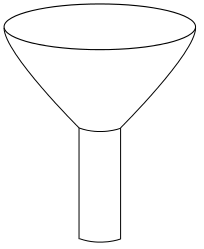
\includegraphics[width=0.25\textwidth]{FIGURES/FilterArray/Filter} & &
\begin{overpic}[scale=.6] %, grid,tics=10]% 
 {FIGURES/Filter}
 \put(20, 70){--, B, --, D, --, --}
\end{overpic} \\
$\Downarrow$ & & $\Downarrow$\\
B & & D \\
\end{tabular}\\
\caption{Example of the two developed arrays}\label{tab:filter}

\end{figure}%